Conclusa la presentazione dell'approccio adottato nelle sperimentazioni, si procede in questo capitolo con l'esposizione dei risultati ottenuti. 

La macchina utilizzata nella risoluzione delle diverse istanze in questi esperimenti presenta le seguenti specifiche tecniche:
\begin{itemize}
\item Intel(R) Xeon(R) CPU E5-2623 v3 @ 3.00GHz quad-core
\item 16GB RAM
\item Python 3.6.8
\item IBM ILOG CPLEX Optimization Studio versione 12.9
\end{itemize}

\newpage
\section{Risultati per grafi $G(n,p)$}
La prima categoria di grafi di cui sono stati analizzati i risultati sono i grafi $G(n,p)$, generati utilizzando il modello di Erdős–Rényi (esposta nella Sottosezione \ref{subsec:er}).

Per prima cosa è stata studiata la correlazione tra la probabilità di generazione di ogni arco e il tempo impiegato da CPLEX nella soluzione dell'istanza del problema di vertex cover, per ciascuno dei parametri di dimensione utilizzati. Per fare questo è stato disegnato un grafico, riportato di seguito in Figura \ref{fig:gnp2d}.
\vspace{-0.5cm}
\begin{figure}[h!]
     \centering
       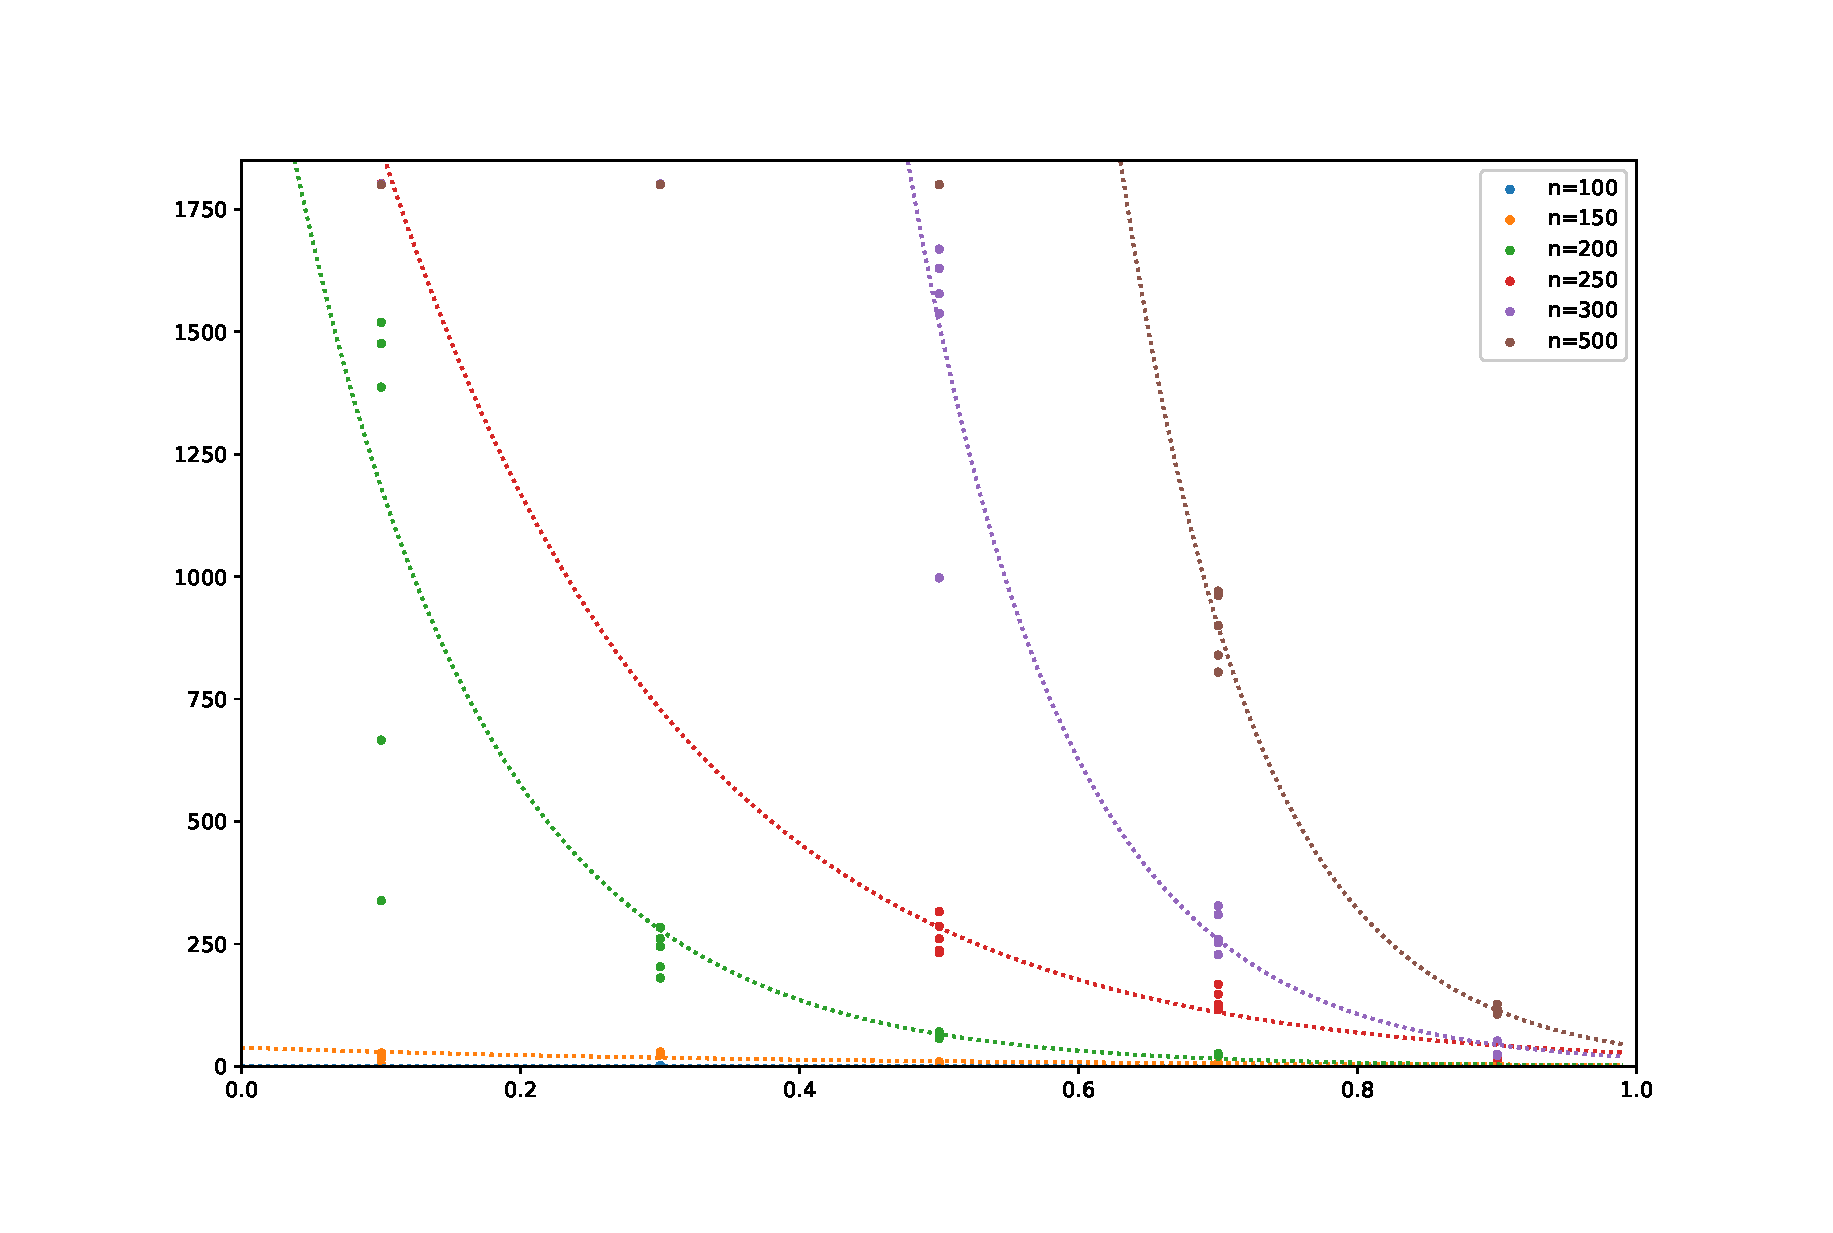
\includegraphics[scale=0.4]{images/gnp-2d.eps}
       \caption{Correlazione tra tempo di risoluzione $time$ (ordinata) e probabilità di generazione di ciascun arco $p$ (ascissa).}
        \label{fig:gnp2d}
\end{figure}

Oltre al semplice plot dei dati, in questo grafico è stata estrapolata una curva da ciascuno degli insiemi di misurazioni corrispondenti ad ogni dimensione (applicando la regressione lineare), in modo tale da riuscirne ad approssimare l'andamento. La regressione è naturalmente stata fatta esclusivamente per le misurazioni di $time$ inferiori al time limit. Il grafico risultante evidenzia una chiara relazione di tipo esponenziale inverso tra $p$ e $time$, per qualsiasi valore del parametro grandezza utilizzato. 

Anche la dimensione dell'istanza di grafo sembra giocare un ruolo relativamente importante nella determinazione della complessità del problema di vertex cover associato, essendo apparentemente responsabile per la velocità con cui l'esponenziale satura.
Per approfondire meglio il ruolo della dimensione nella determinazione della complessità di risoluzione si è rappresentato graficamente l'andamento del tempo di risoluzione al variare della dimensione del grafo e a parità di valori del parametro $p$. I risultati ottenuti sono riportati in Figura \ref{fig:gnpp}.

\begin{figure}[h!]
     \centering
       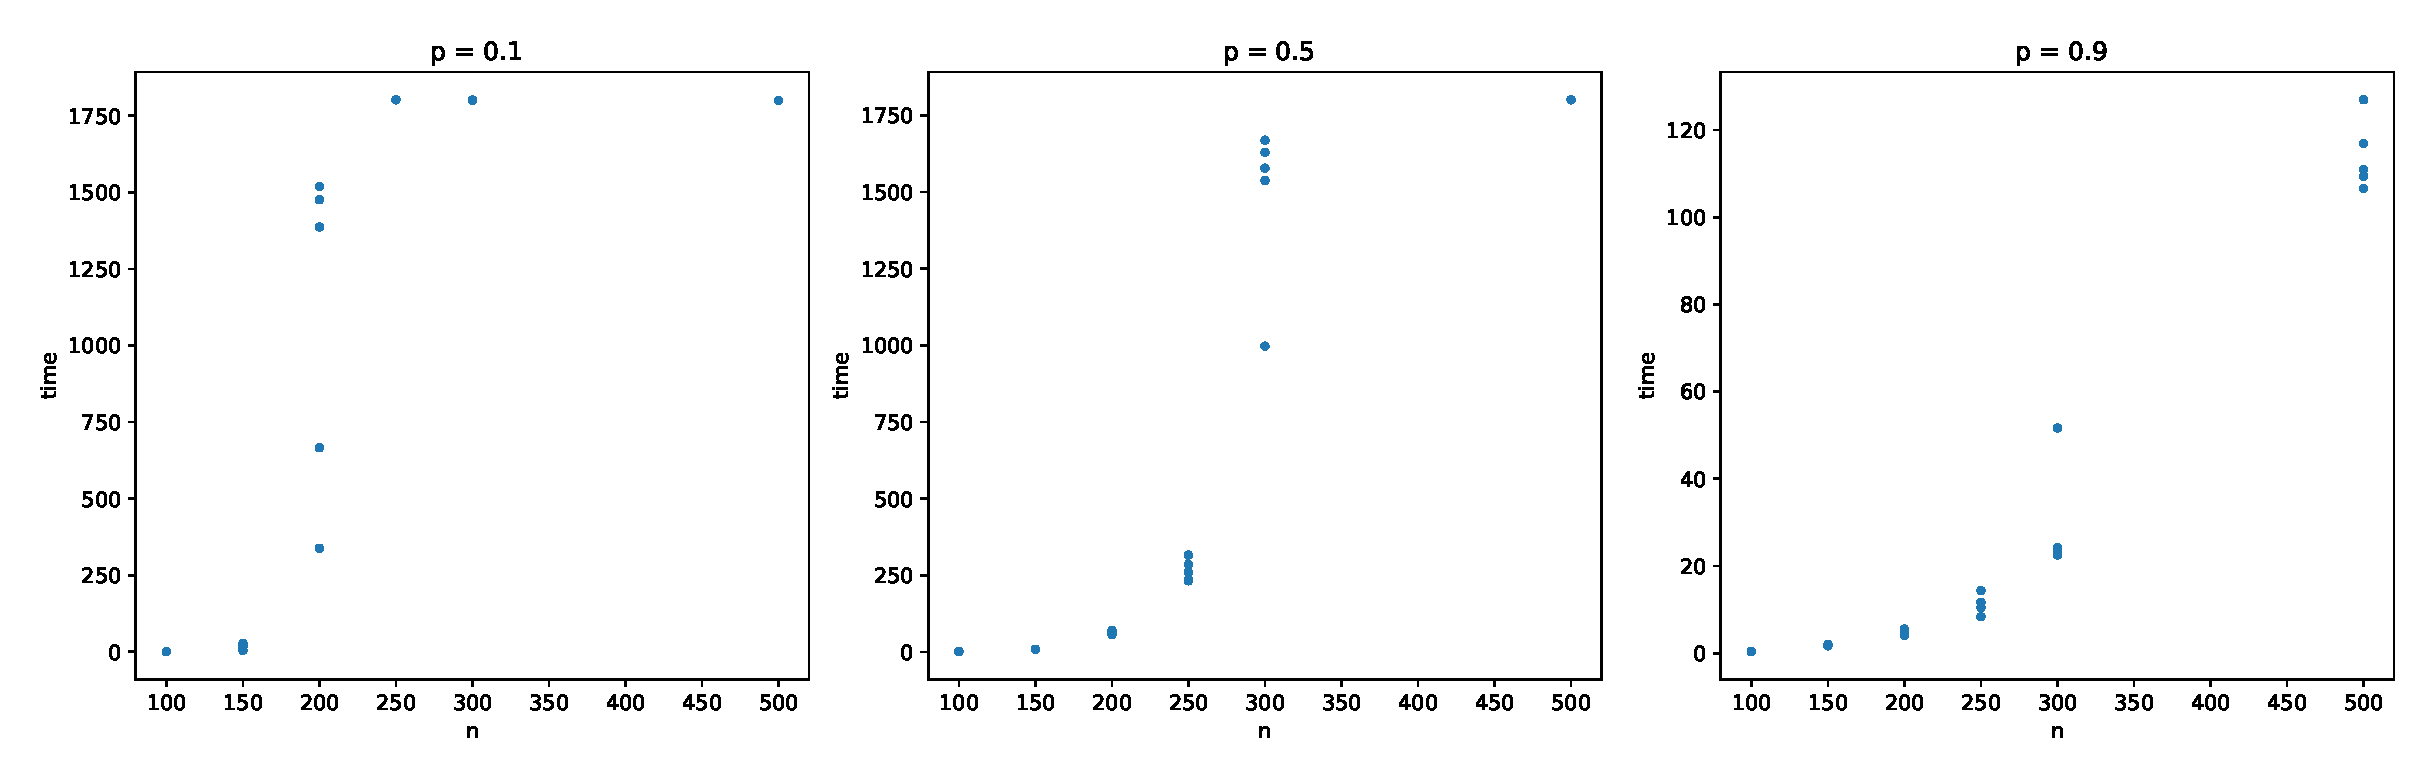
\includegraphics[scale=0.4]{images/gnp_p.eps}
       \caption{Correlazione tra tempo di risoluzione $time$ (ordinata) e dimensione del grafo $n$ (ascissa) per diversi valori di probabilità fissata $p=0.1$, $p=0.5$ e $p=0.9$.}
        \label{fig:gnpp}
\end{figure}

Come si può evincere dal grafo precedente, istanze di grafi più grandi diventano computazionalmente intrattabili molto prima rispetto a istanze dalla dimensione più contenuta, a parità di $p$. Tuttavia, come dimostra il grafico in Figura \ref{fig:gnpp} ottenuto per $p=0.9$,  il contributo dato dal numero di nodi alla complessità di risoluzione sembra essere secondario rispetto al ruolo giocato dalla probabilità di generazione di ogni arco $p$. 

In Figura \ref{fig:gnp3d} viene infine riportato un grafico tridimensionale riassuntivo, che rappresenta in un'unica immagine il variare della complessità del problema rispetto ad entrambi i parametri utilizzati nella generazione del grafo.
\vspace{-1cm}
\begin{figure}[h!]
     \centering
       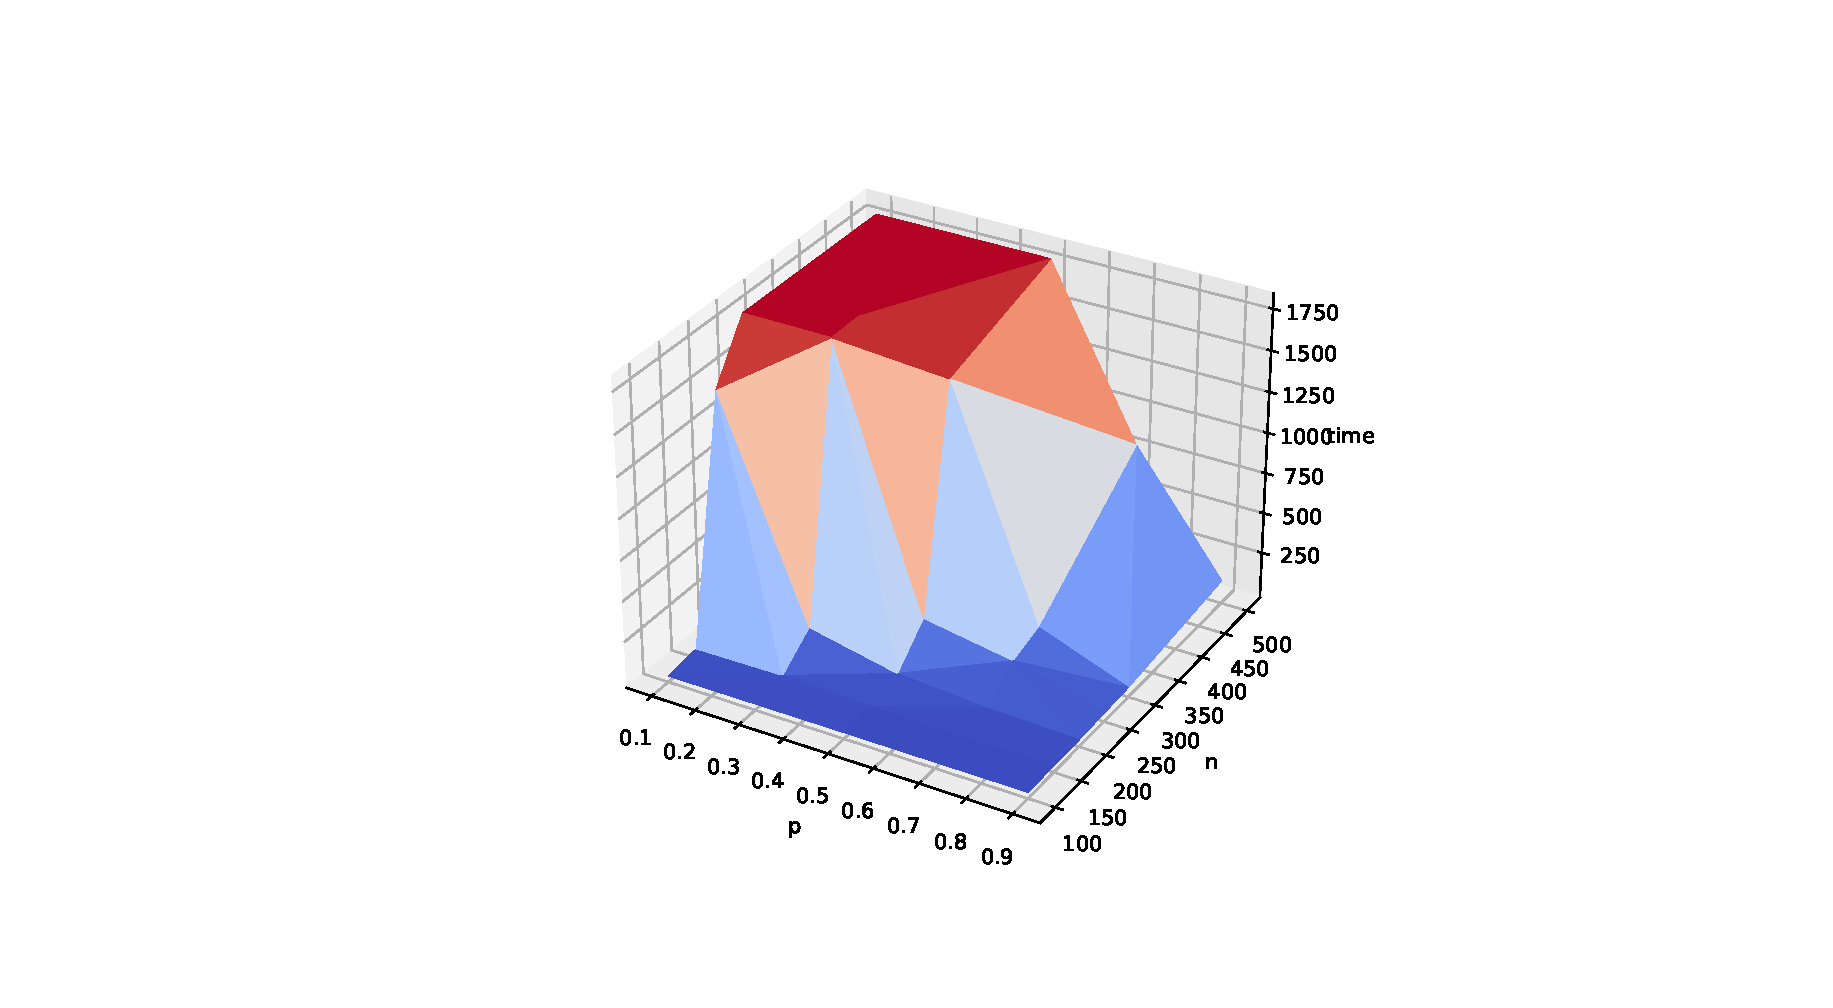
\includegraphics[scale=0.5]{images/gnp-3d.eps}
       \vspace{-0.8cm}
       \caption{Rappresentazione tridimensionale dell'andamento della complessità del problema di vertex cover per grafi $G(n,p)$ al variare dei parametri $p$ ed $n$.Colori più caldi indicano una complessità maggiore ed il colore rosso scuro è generalmente sinonimo di raggiungimento del time limit imposto al risolutore}
        \label{fig:gnp3d}
\end{figure}


\section{Risultati per grafi regolari}
La seconda categoria di grafi per cui è stato studiato l'andamento della complessità computazionale è stata quella dei grafi regolari, generati secondo il modello di Steger-Wormald già descritto nella Sottosezione \ref{subsec:steger}.

In questo caso, una prima analisi è stata fatta sull'andamento della complessità computazionale del problema di vertex cover associato al variare del grado di ciascun nodo $d$, per ognuna delle dimensioni di grafo specificate. Il grafico risultante da questa analisi è riportato in Figura \ref{fig:rrgd}. A differenza dei grafi $G(n,p)$, in cui a parità di parametri di generazione $n$ e $p$ il tempo di risoluzione dimostrava oscillazioni quasi trascurabili per i diversi semi utilizzati nella gestione del comportamento casuale, nel caso dei grafi regolare le oscillazioni tra istanze generate a partire da semi diversi sono risultate essere molto marcate. Per questa ragione è stato considerato per ognuna delle coppie $(n,d)$ il valore medio del tempo di risoluzione. 
\vspace{-1cm}
\begin{figure}[h!]
     \centering
       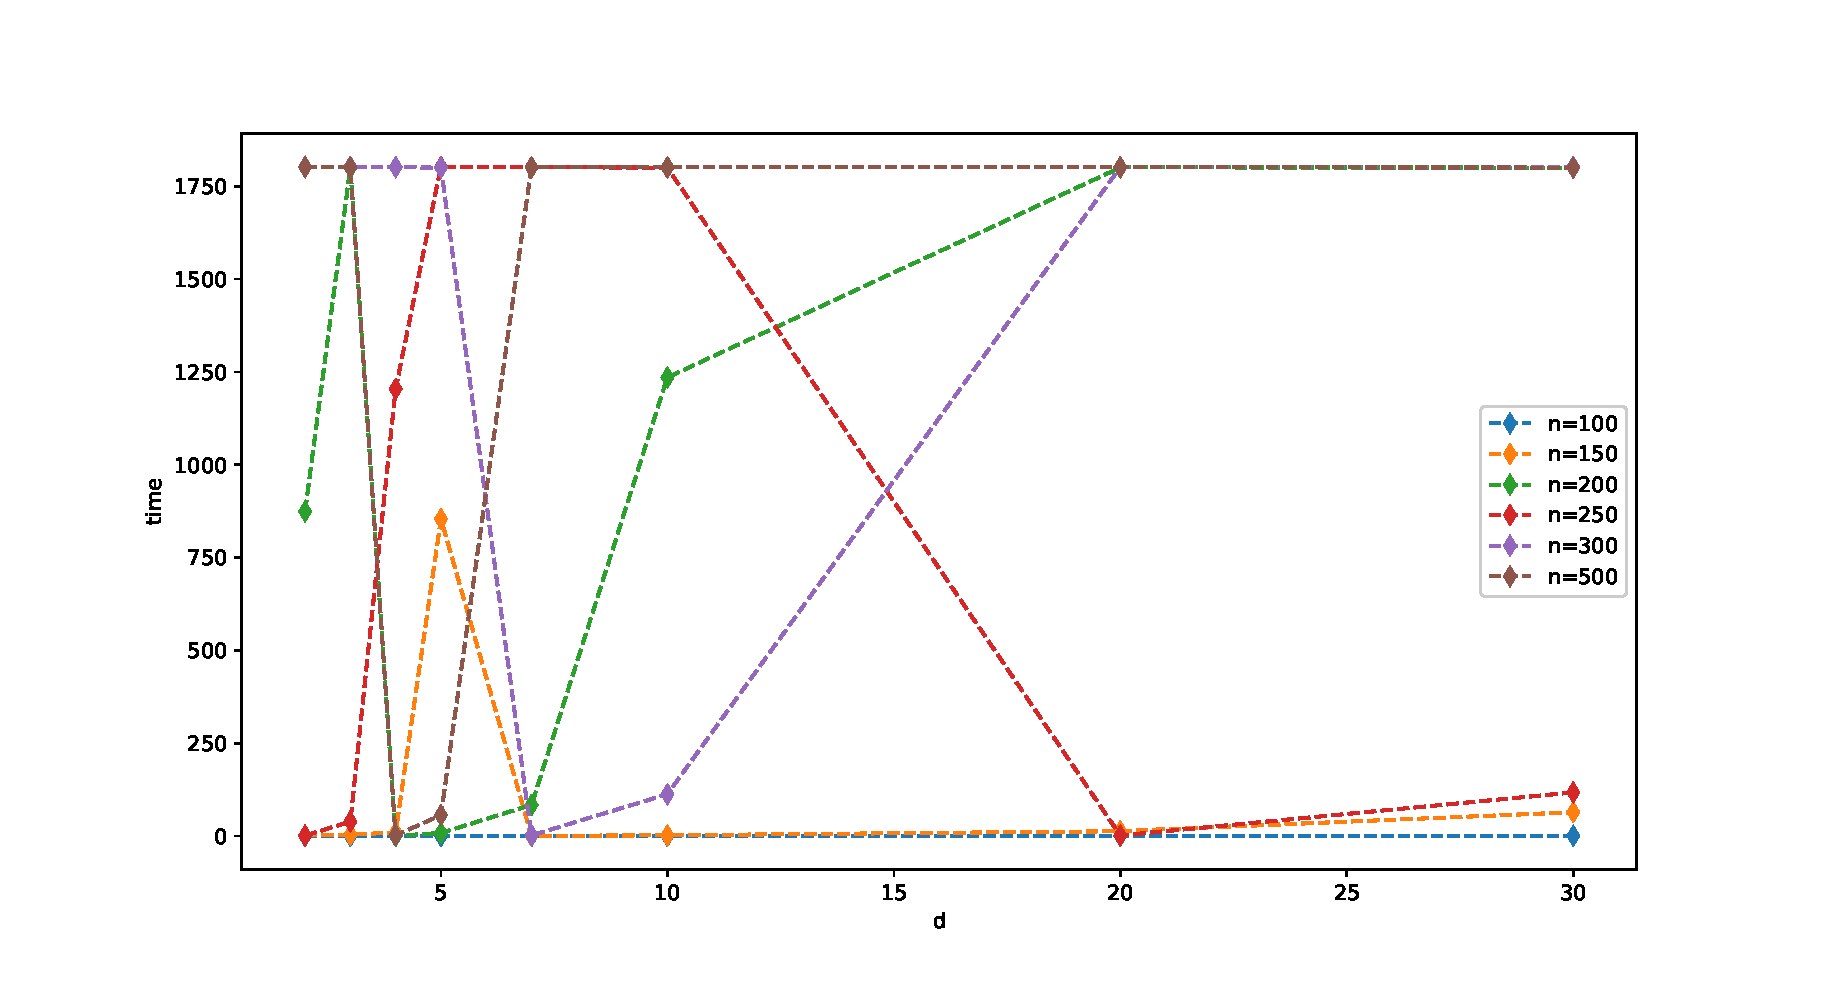
\includegraphics[scale=0.5]{images/rrg-d.eps}
       \caption{Andamento della complessità del problema di vertex cover per grafi regolari al variare del grado di ciascun nodo $d$, per diversi valori di dimensione $n$.}
        \label{fig:rrgd}
\end{figure}

In questo caso risulta molto difficile, se non impossibile, riuscire a trovare un pattern ricorrente nei comportamenti delle diverse istanze. Una debole ipotesi sulla correlazione tra dimensione del grafo e complessità del problema potrebbe essere avanzata per questa particolare tipologia di grafi, sebbene esistano due valori di dimensione ($n=200$ e $n=250$) che si comportano esattamente al contrario di quanto previsto. Questa anomalia potrebbe essere tuttavia dovuta al fatto che i due valori di dimensione si trovano in una zona di confine, in cui il comportamento della complessità del problema è instabile e viene fortemente influenzato dalla forma delle specifiche istanze.

Una proprietà comune alle istanze di tutte le dimensioni (escluse quelle di dimensione più piccola generate per $n=100$) sembra poi essere un'inversione di tendenza della complessità del problema (sia in meglio che in peggio) in una finestra di valori del parametro $d$ compresa tra 3 e 10. Questo fenomeno fa si che istanze di grande dimensione che per tutti gli altri valori di $d$ risultano perennemente irrisolvibili diventino molto facili e, al contrario, istanze di piccola dimensione che risultano essere sempre risolte in tempi molto piccoli vadano invece in time limit. Una rappresentazione tridimensionale dell'andamento della complessità al variare dei due parametri in contemporanea, che permette di apprezzare meglio questo fenomeno, è riportata in Figura \ref{fig:rrg3d}.

\begin{figure}[h!]
     \centering
       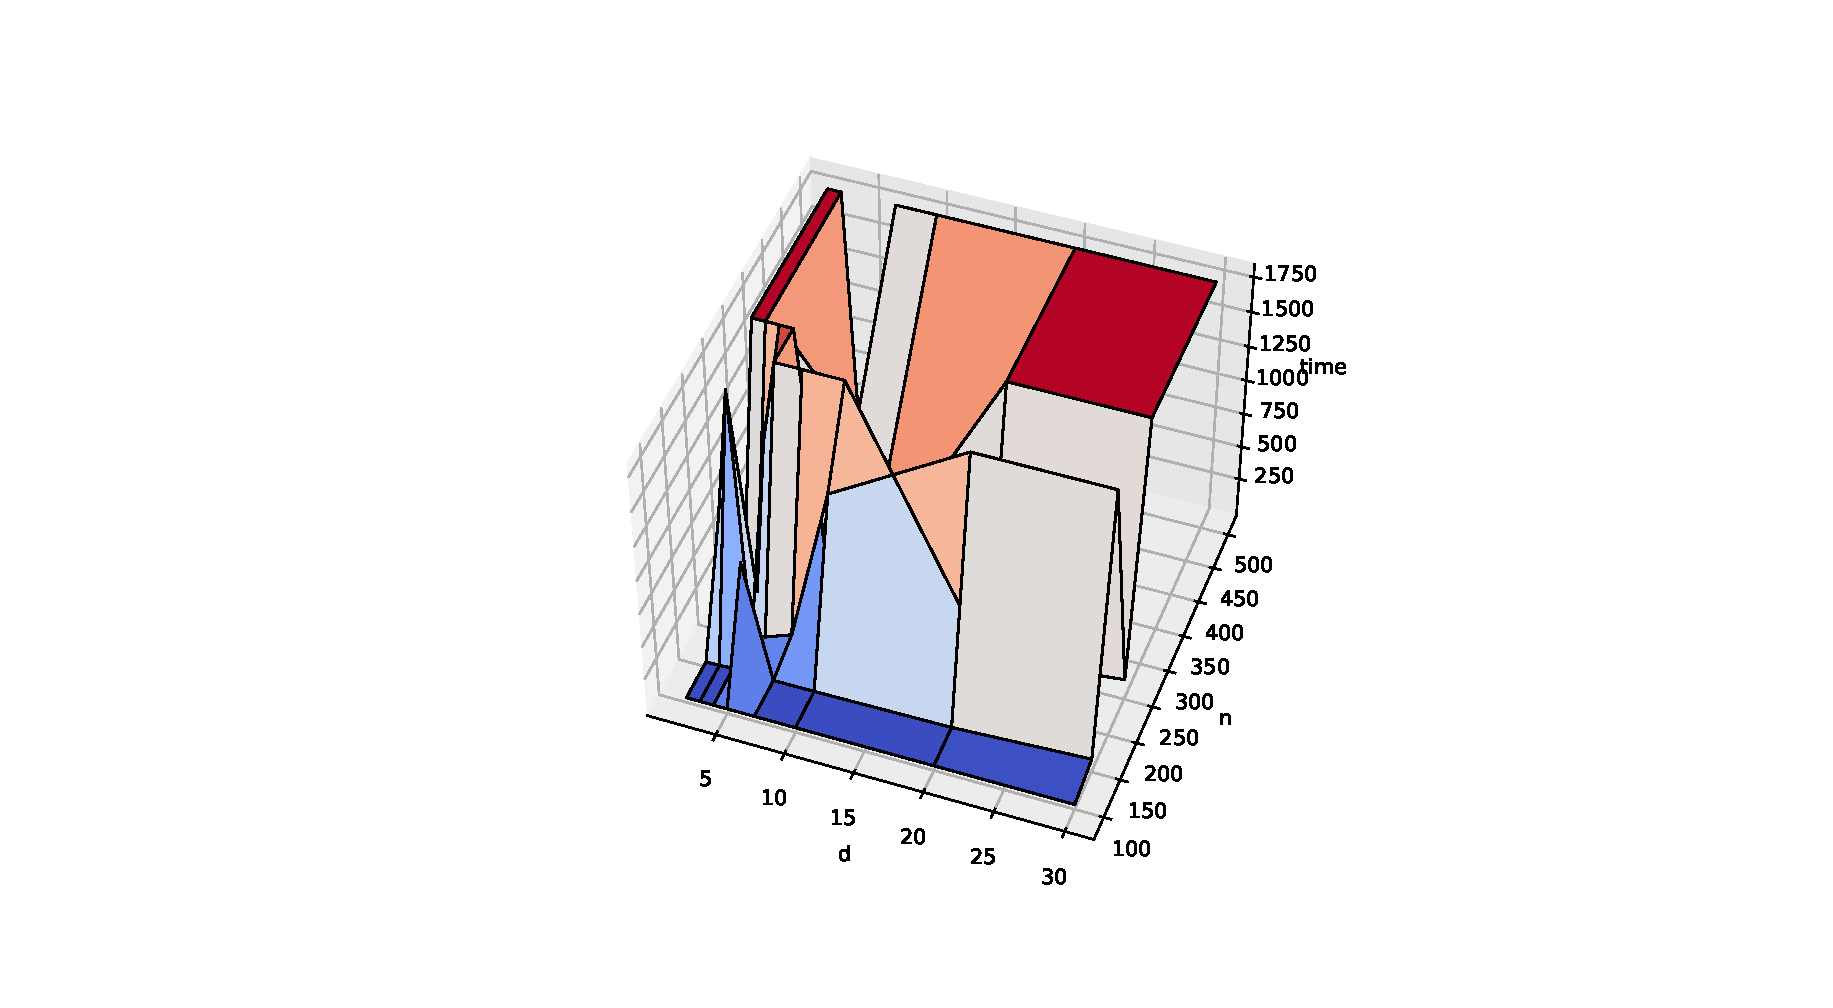
\includegraphics[scale=0.5]{images/rrg3d.eps}
       \caption{Rappresentazione tridimensionale dell'andamento della complessità del problema di vertex cover per grafi regolari al variare dei parametri $d$ ed $n$. Anche in questo caso colori più caldi indicano una complessità maggiore, ed il colore rosso scuro è generalmente sinonimo di raggiungimento del time limit imposto al risolutore}      
        \label{fig:rrg3d}
\end{figure}

Anche in questo caso, dare una spiegazione a questo fenomeno risulta molto complicato e sarebbe necessaria un'analisi più approfondita sulla forma delle specifiche istanze dei grafi e sullo sulle loro proprietà.

\section{Risultati per grafi di Watts-Strogatz}

\newpage
\section{Risultati per grafi di Barabási-Albert}
L'ultima categoria di grafi di cui sono stati studiati i risultati sperimentali sono stati quelli generati mediante il modello di Barabási-Albert, già trattato nella Sottosezione \ref{subsec:barab}. 

Per prima cosa è stata analizzata la correlazione tra dimensione del grafo e complessità nella risoluzione del problema, estrapolando una curva per ognuno degli insiemi di misurazioni legate ad uno specifico valore del parametro $d$.  L'andamento ottenuto si è dimostrato essere marcatamente esponenziale (crescente). È stato possibile anche in questo caso applicare il metodo della regressione lineare al fine di ottenere delle curve in grado di approssimare sufficientemente bene l'andamento del tempo impiegato dal risolutore ad ottenere una soluzione.Il grafico che è risultato da questo studio dei risultati è riportato in Figura \ref{fig:bag1}.
\vspace{-0.5cm}  
\begin{figure}[h!]
     \centering
       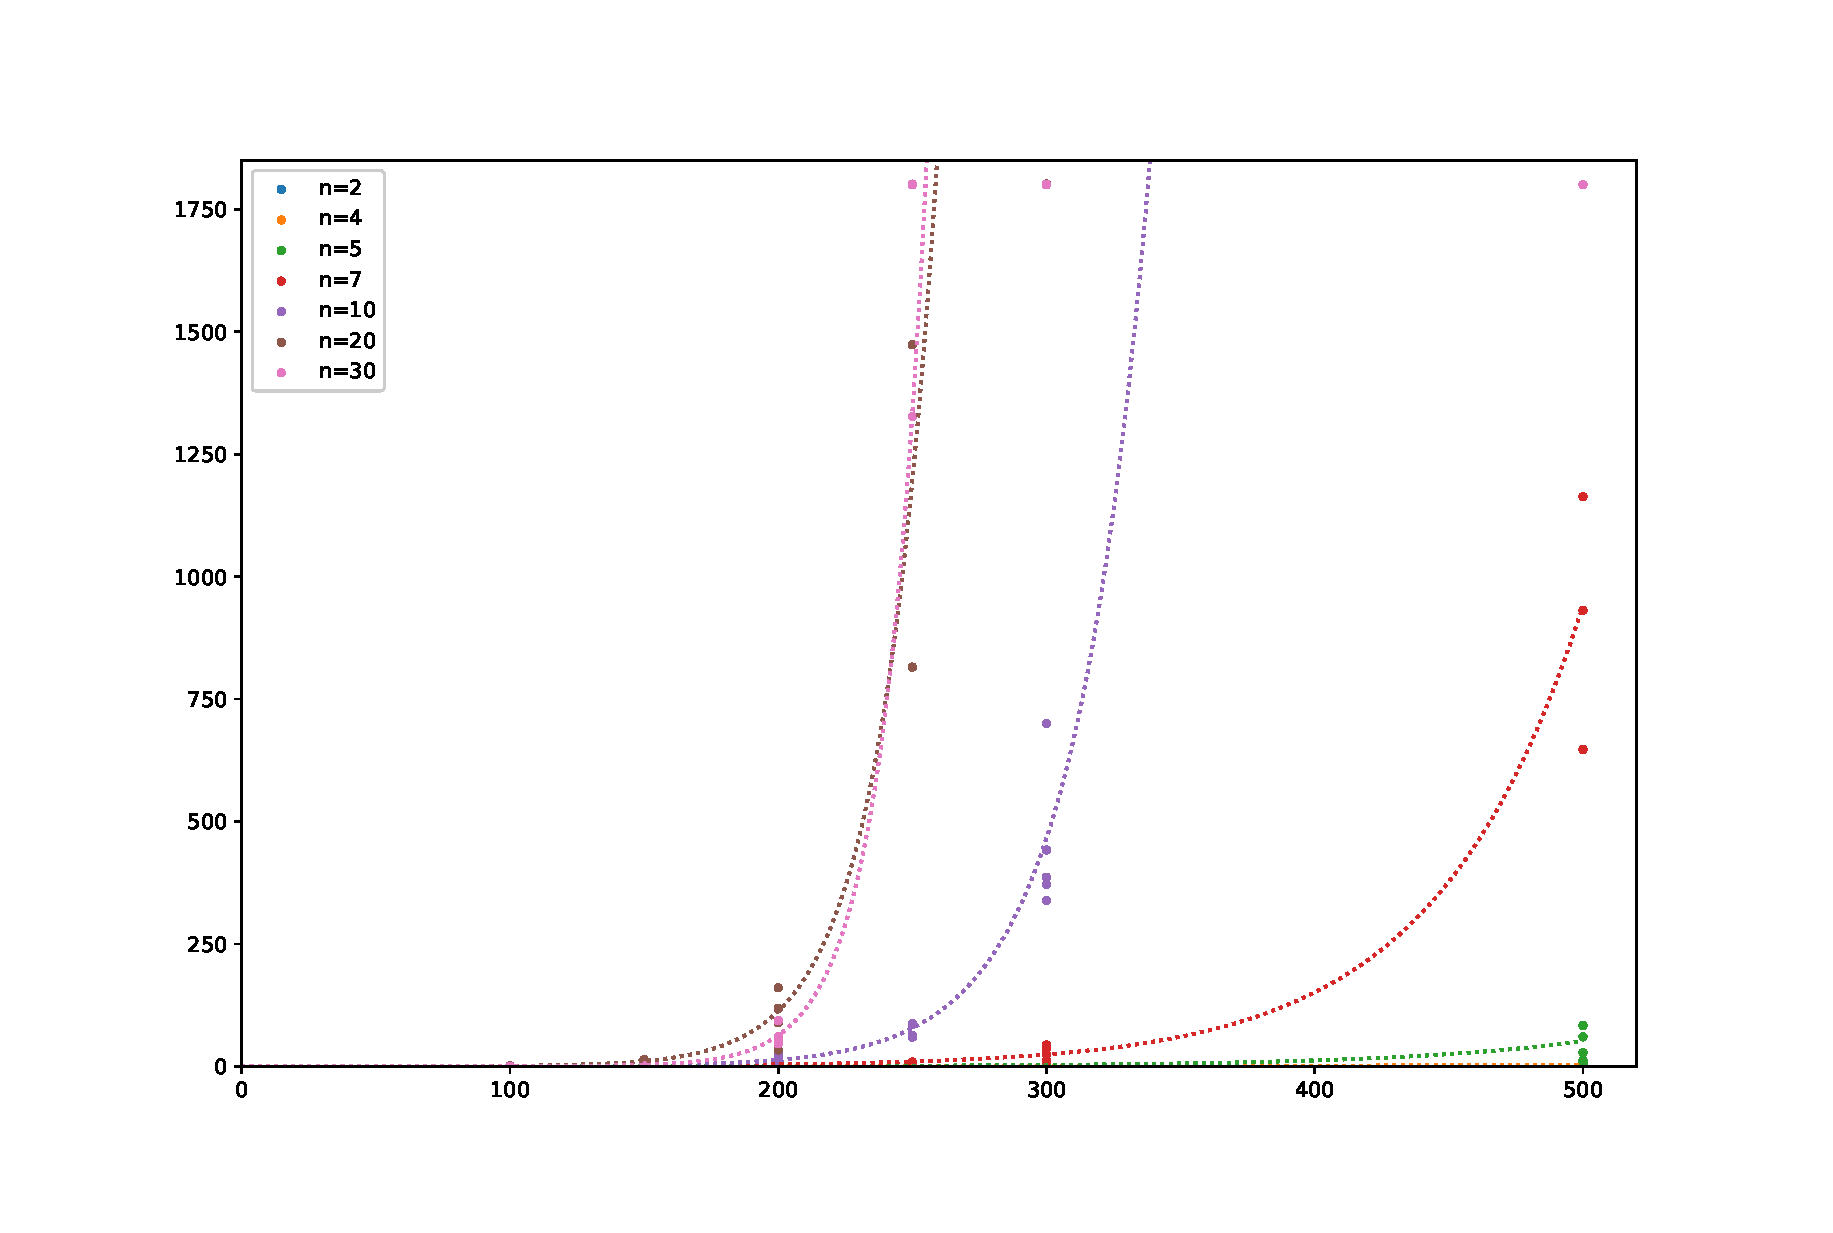
\includegraphics[scale=0.5]{images/bag.eps}
       \vspace{-0.5cm}  
       \caption{Andamento del tempo impiegato da CPLEX per risolvere l'istanza di problema (ordinata) in funzione della grandezza del grafo (ascissa), per diversi valori del parametro $m$, corrispondente al numero di archi creati tra ogni nuovo nodo ed i nodi esistenti nel processo di generazione.}      
      
        \label{fig:bag1}
\end{figure}

In seconda istanza è stato analizzato il contributo del parametro $m$, mantenendo questa volta costante il numero dei nodi del grafo. Come si può evincere dai grafici riportati in Figura \ref{fig:bagma}, il parametro $m$ sembra avere un impatto marginale sulla complessità del problema, o almeno non paragonabile a quello determinato dalla dimensione del problema stesso. Valori anche grandi di $m$ infatti non causano mai da soli la divergenza delle tempo di risoluzione, ma al limite la favoriscono nel caso di grafi dalla dimensione marcata. 

È inoltre interessante notare come, per il valore $m=30$, il tempo di risoluzione sia mediamente inferiore (per le istanze di problema che non vanno in time limit) rispetto al caso $m=20$, in netto contrasto con l'andamento strettamente crescente evidenziato fino a quel momento. Ciò potrebbe essere dovuto ad una particolare configurazione di forma assunta dai grafi per tale valore di $m$ o potrebbe trattarsi invece di una vera e propria inversione di tendenza. In entrambi i casi, uno studio per un insieme molto più esteso di valori del parametro $m$ sarebbe necessario.

\begin{figure}[h!]
     \centering
     \begin{subfigure}[b]{\textwidth}
     	\centering
	     \begin{subfigure}[b]{0.32\textwidth}
	         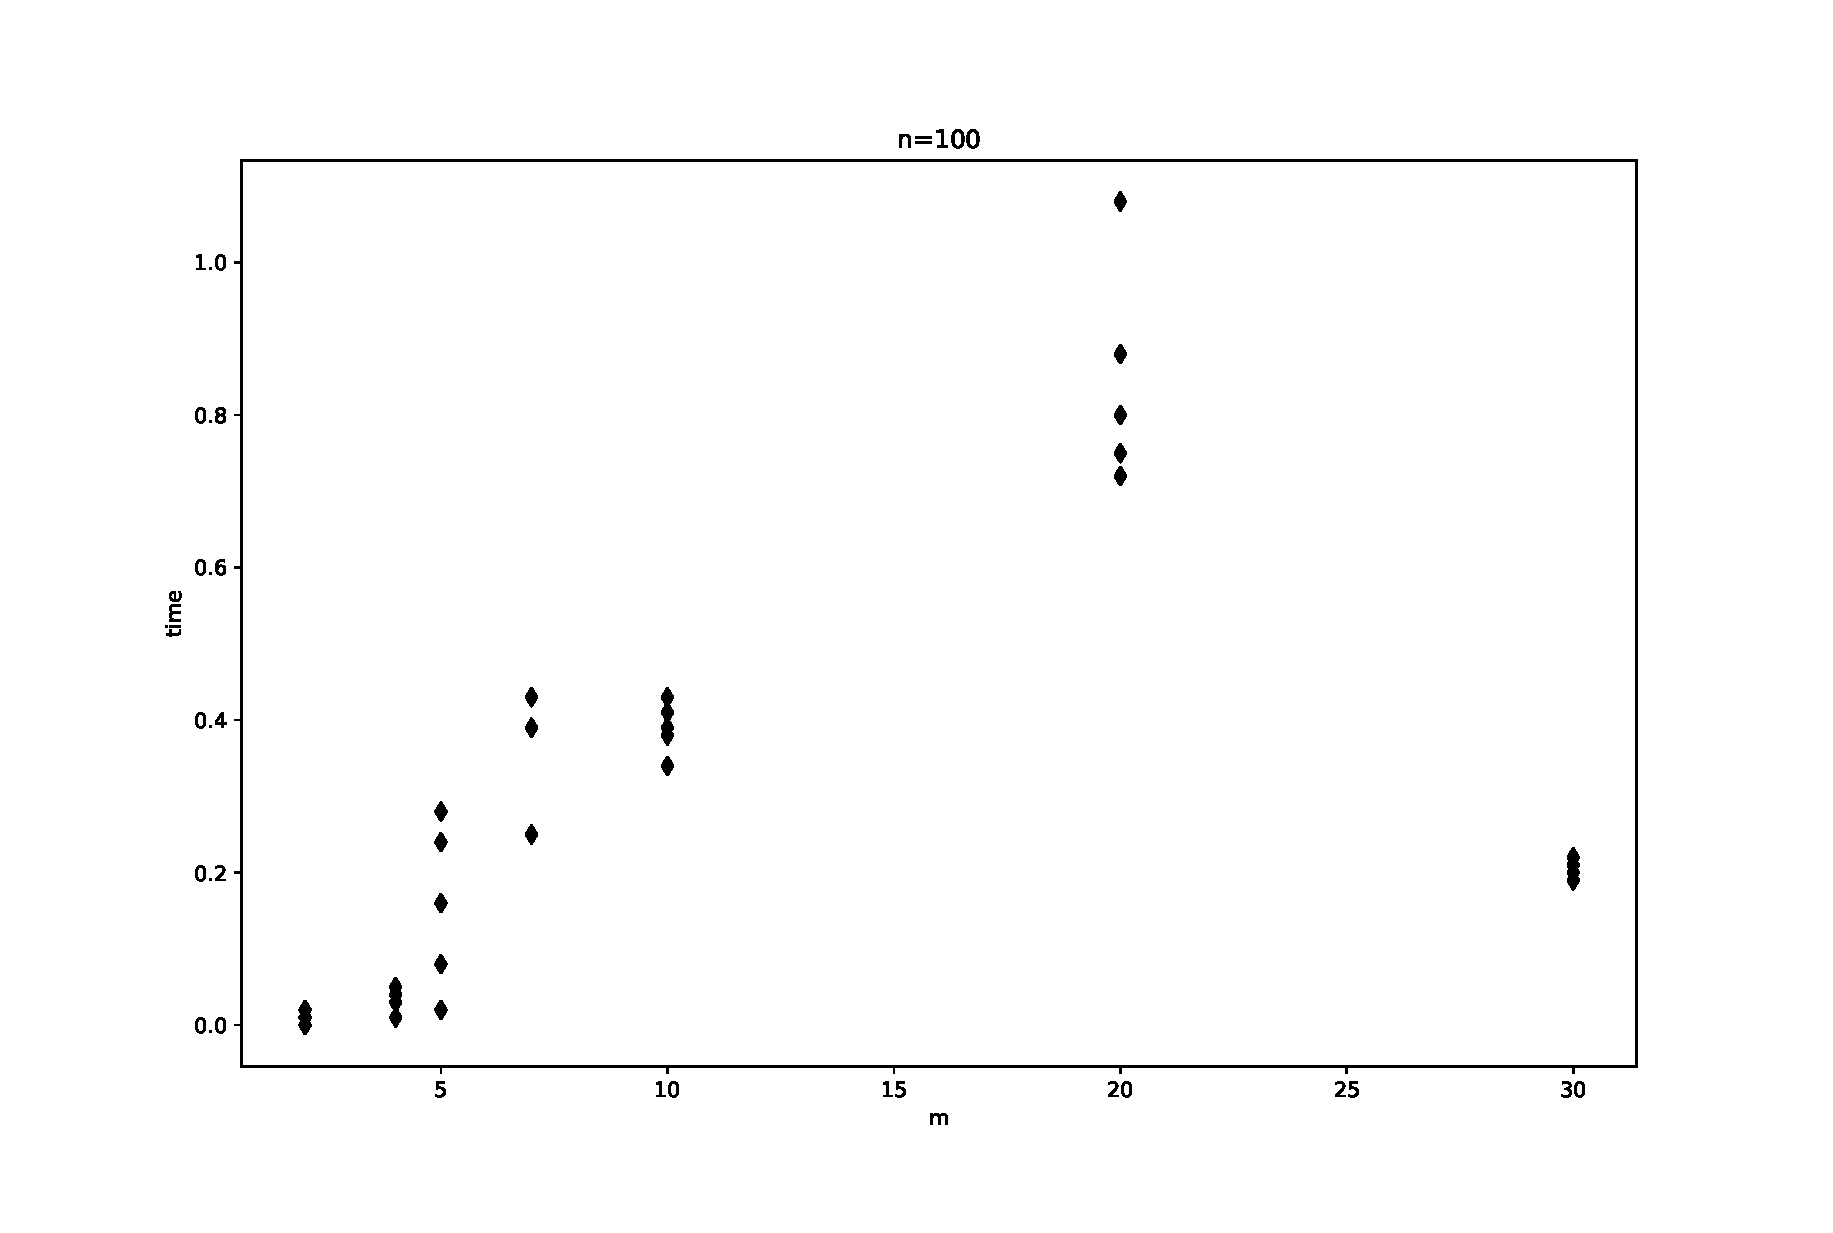
\includegraphics[width=\columnwidth]{images/bagm0.eps}
	     \end{subfigure}
	     \hspace{0em}
	     \begin{subfigure}[b]{0.32\textwidth}
	         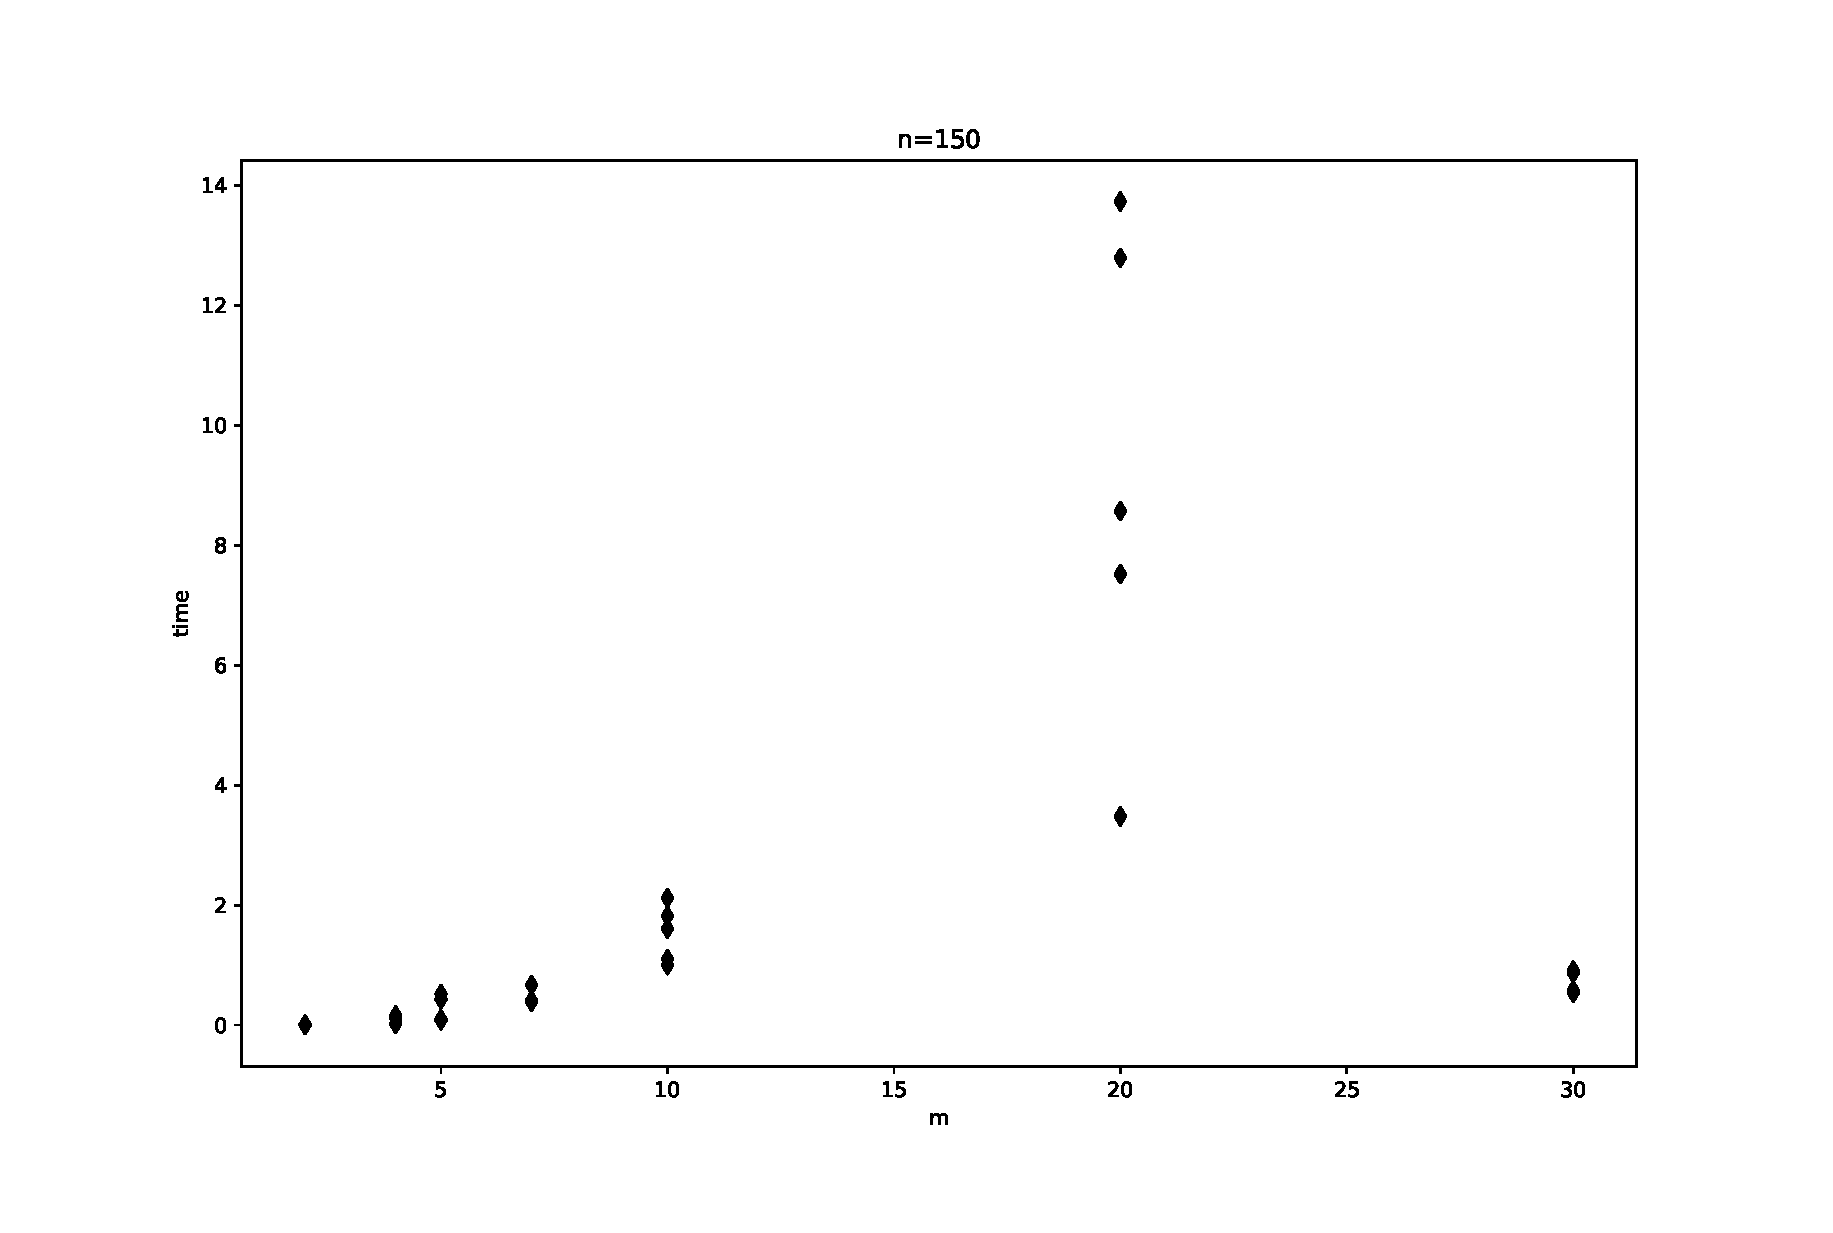
\includegraphics[width=\columnwidth]{images/bagm1.eps}
	     \end{subfigure}
	     \hspace{0em}
	     \begin{subfigure}[b]{0.32\textwidth}
	         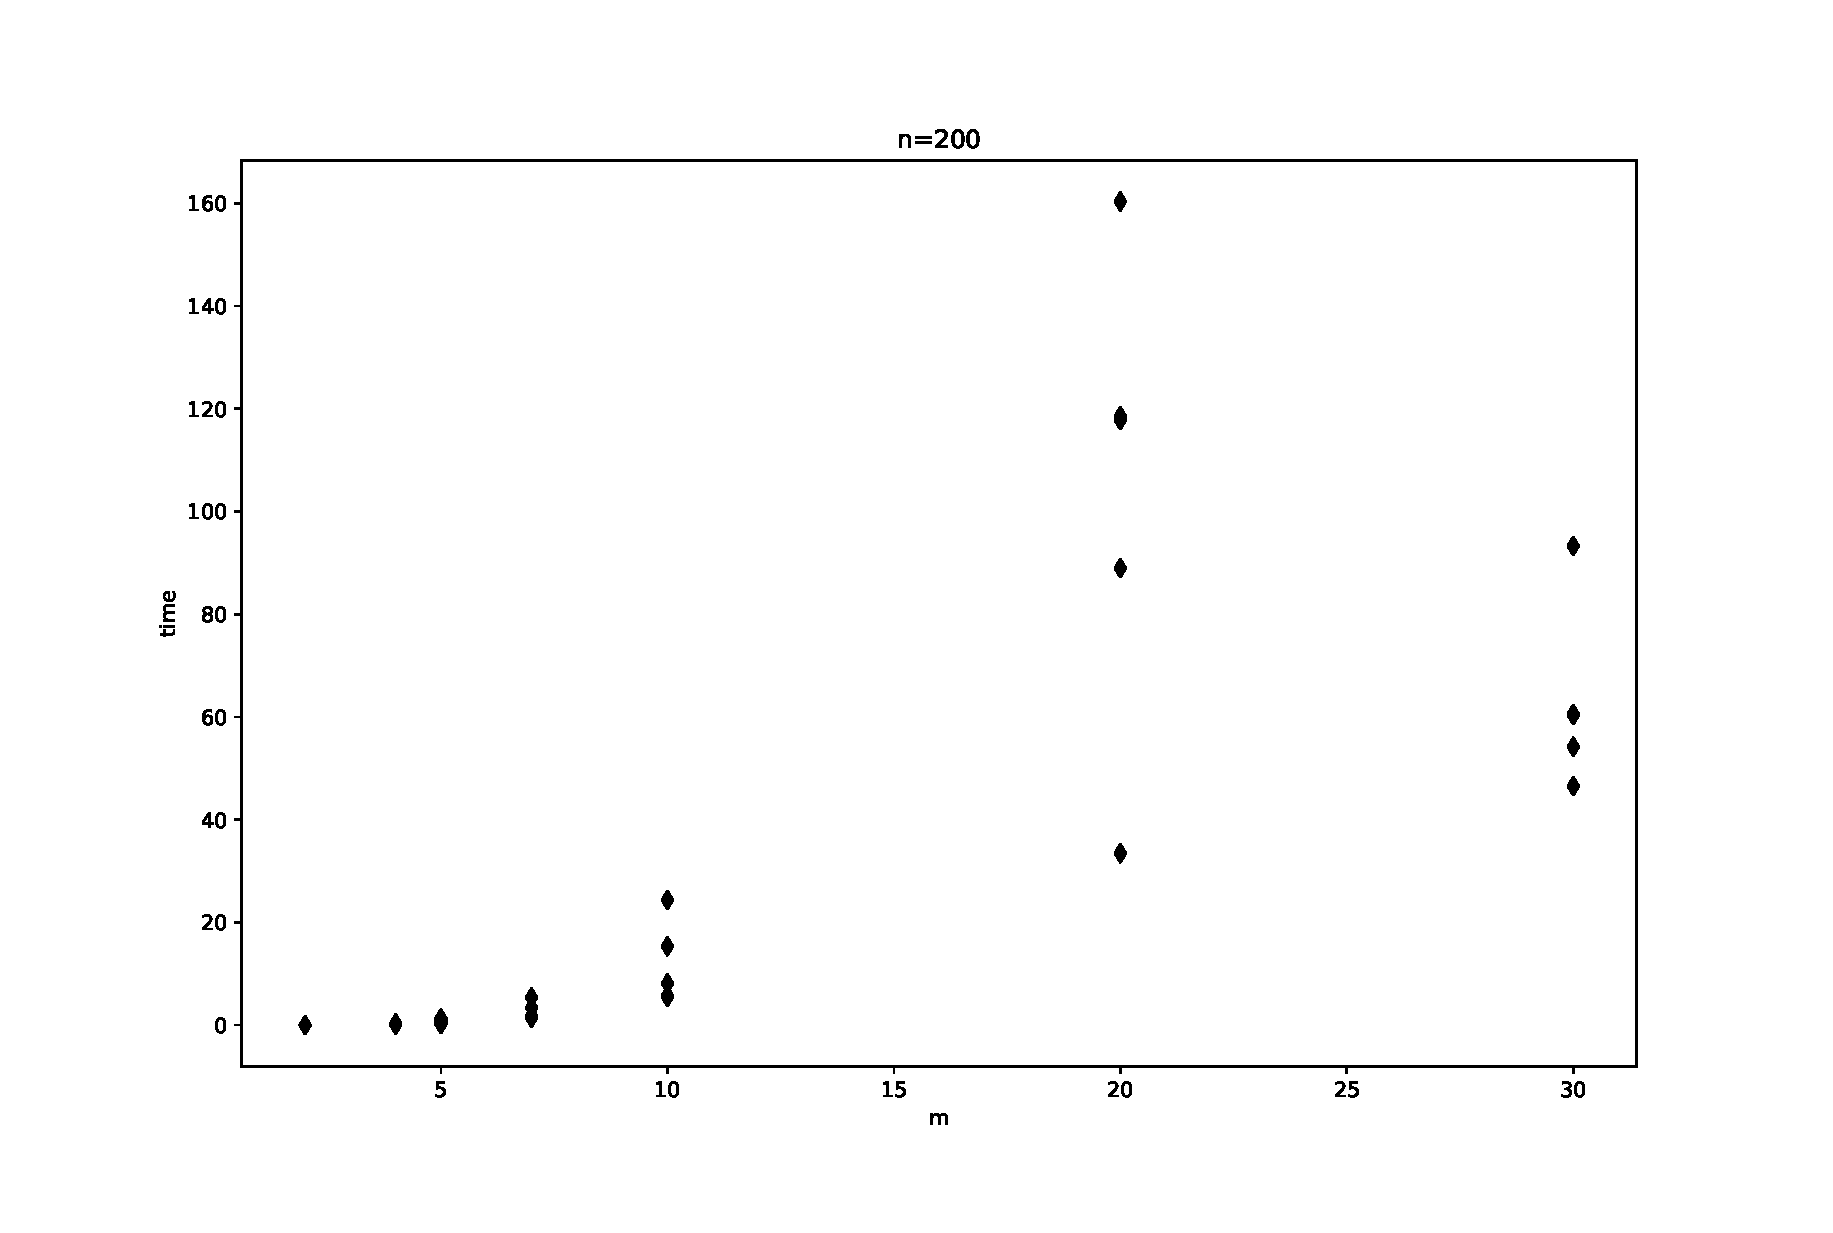
\includegraphics[width=\columnwidth]{images/bagm2.eps}
	     \end{subfigure}
	  \end{subfigure}
	  \begin{subfigure}[b]{\textwidth}
	  	\centering
	      \begin{subfigure}[b]{0.32\textwidth}
	         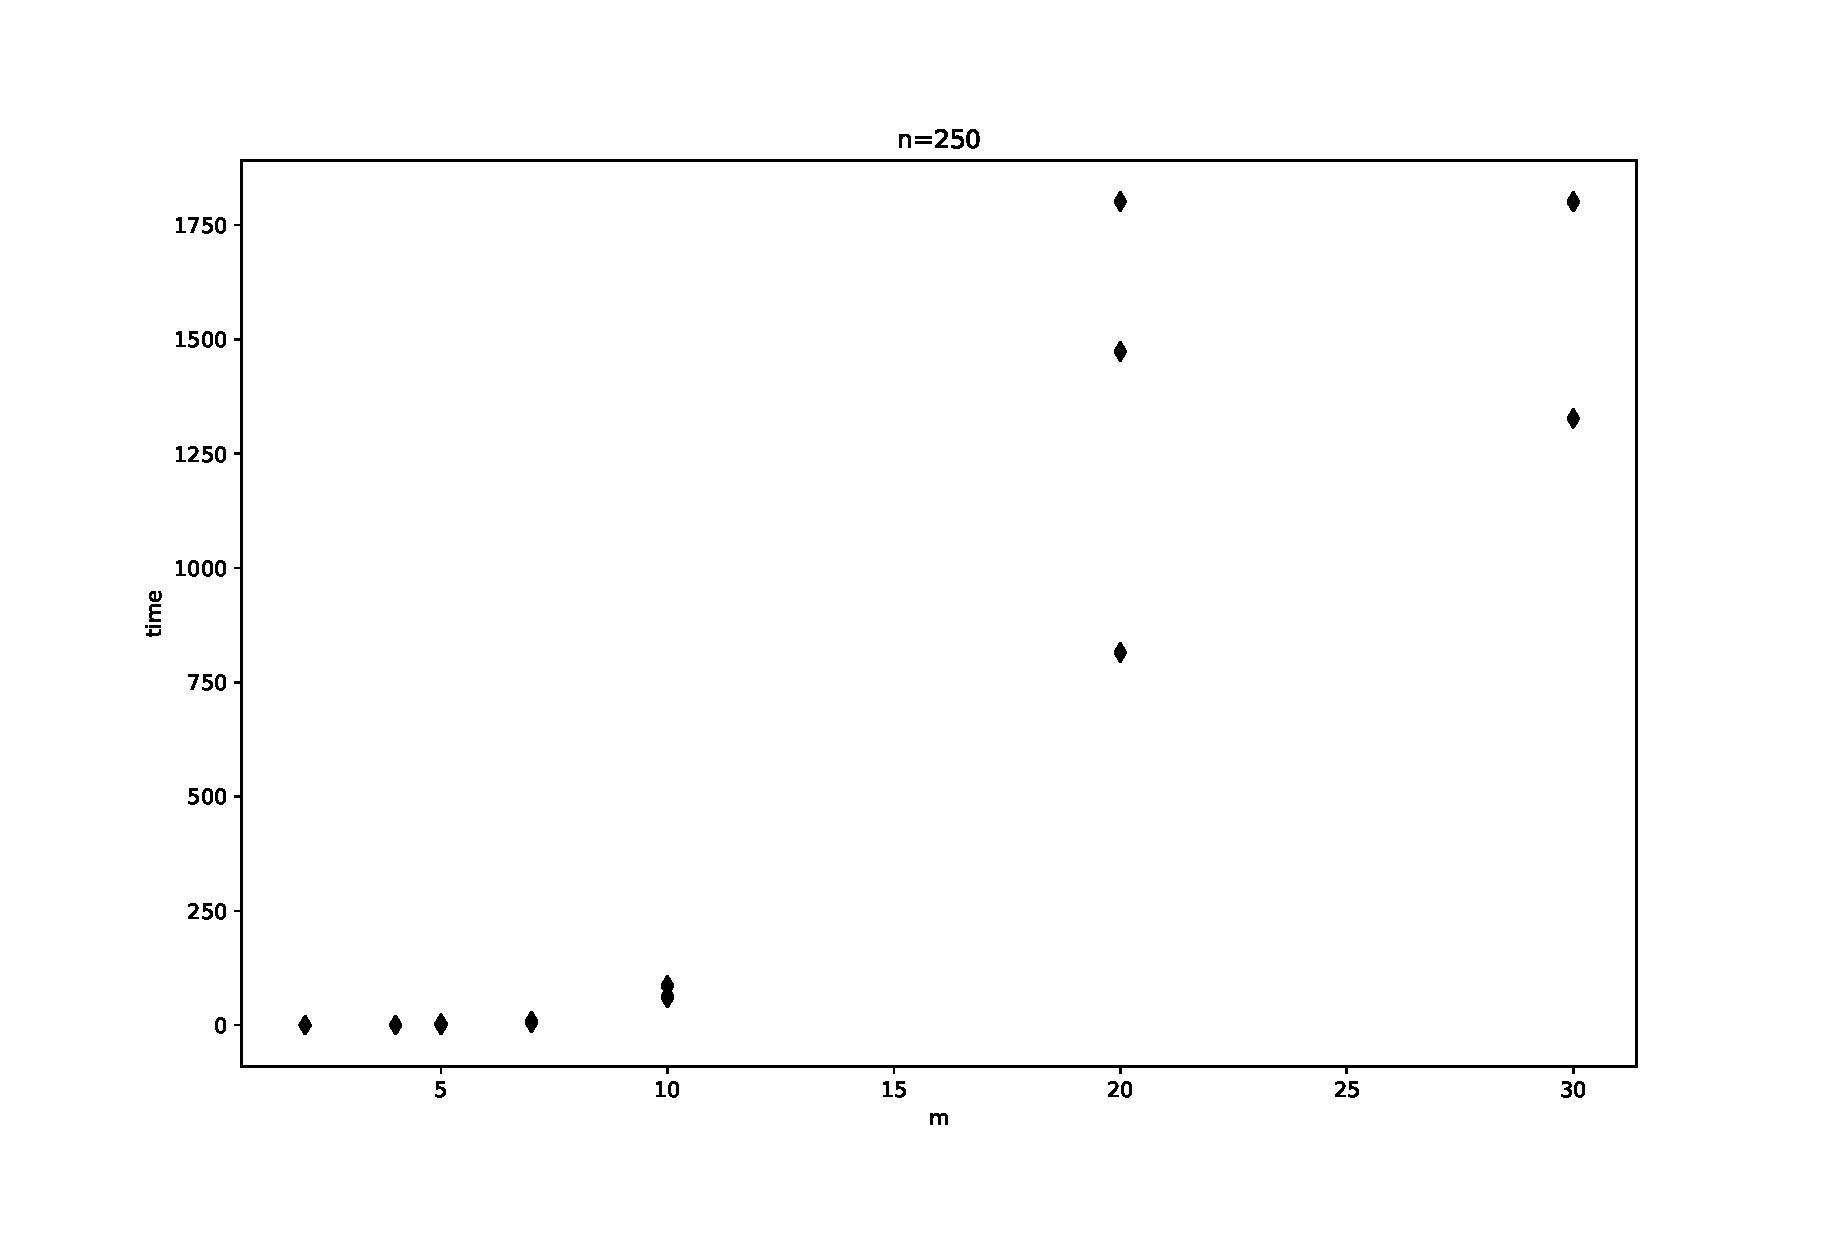
\includegraphics[width=\columnwidth]{images/bagm3.eps}
	     \end{subfigure}
	     \hspace{0em}
	      \begin{subfigure}[b]{0.32\textwidth}
	         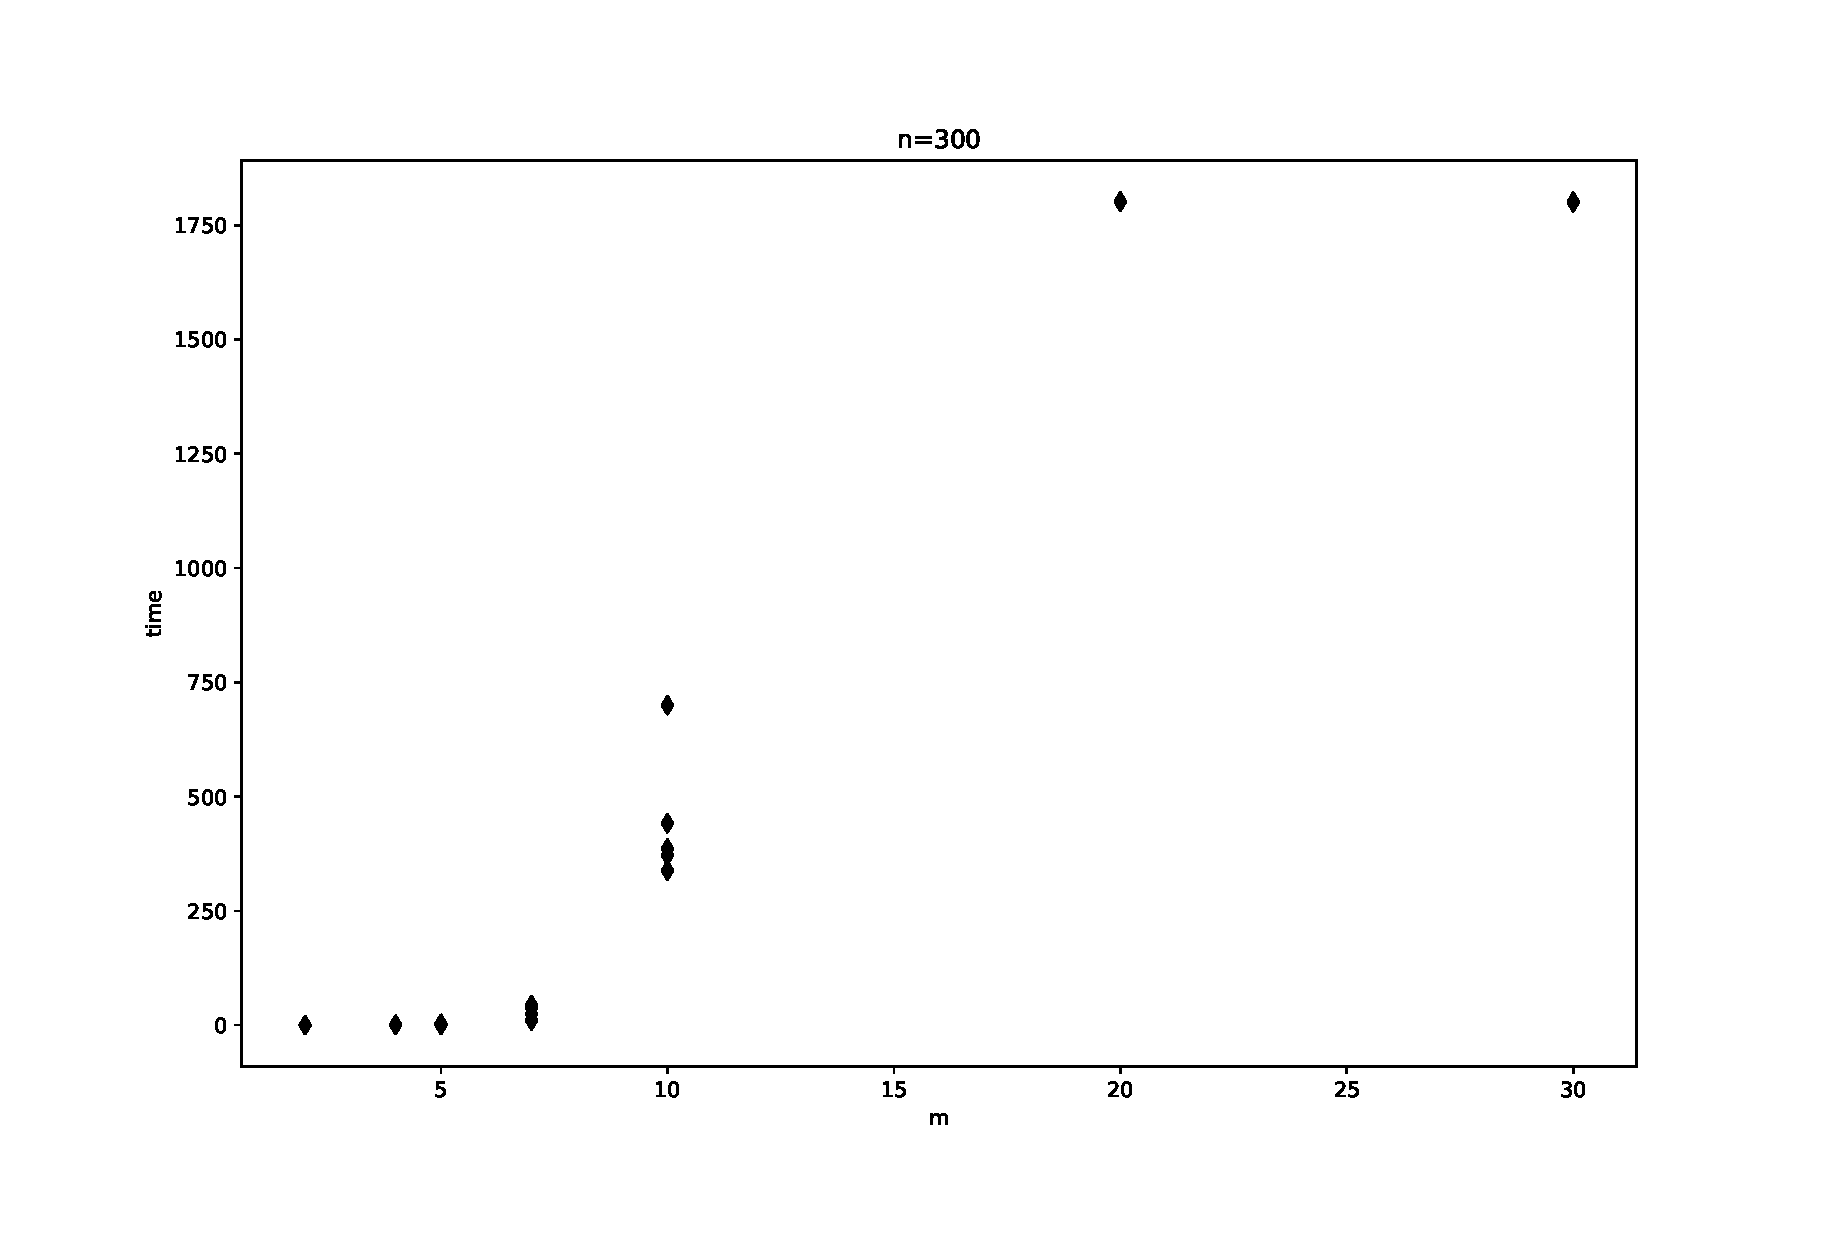
\includegraphics[width=\columnwidth]{images/bagm4.eps}
	     \end{subfigure}
	     \hspace{0em}
	      \begin{subfigure}[b]{0.32\textwidth}
	         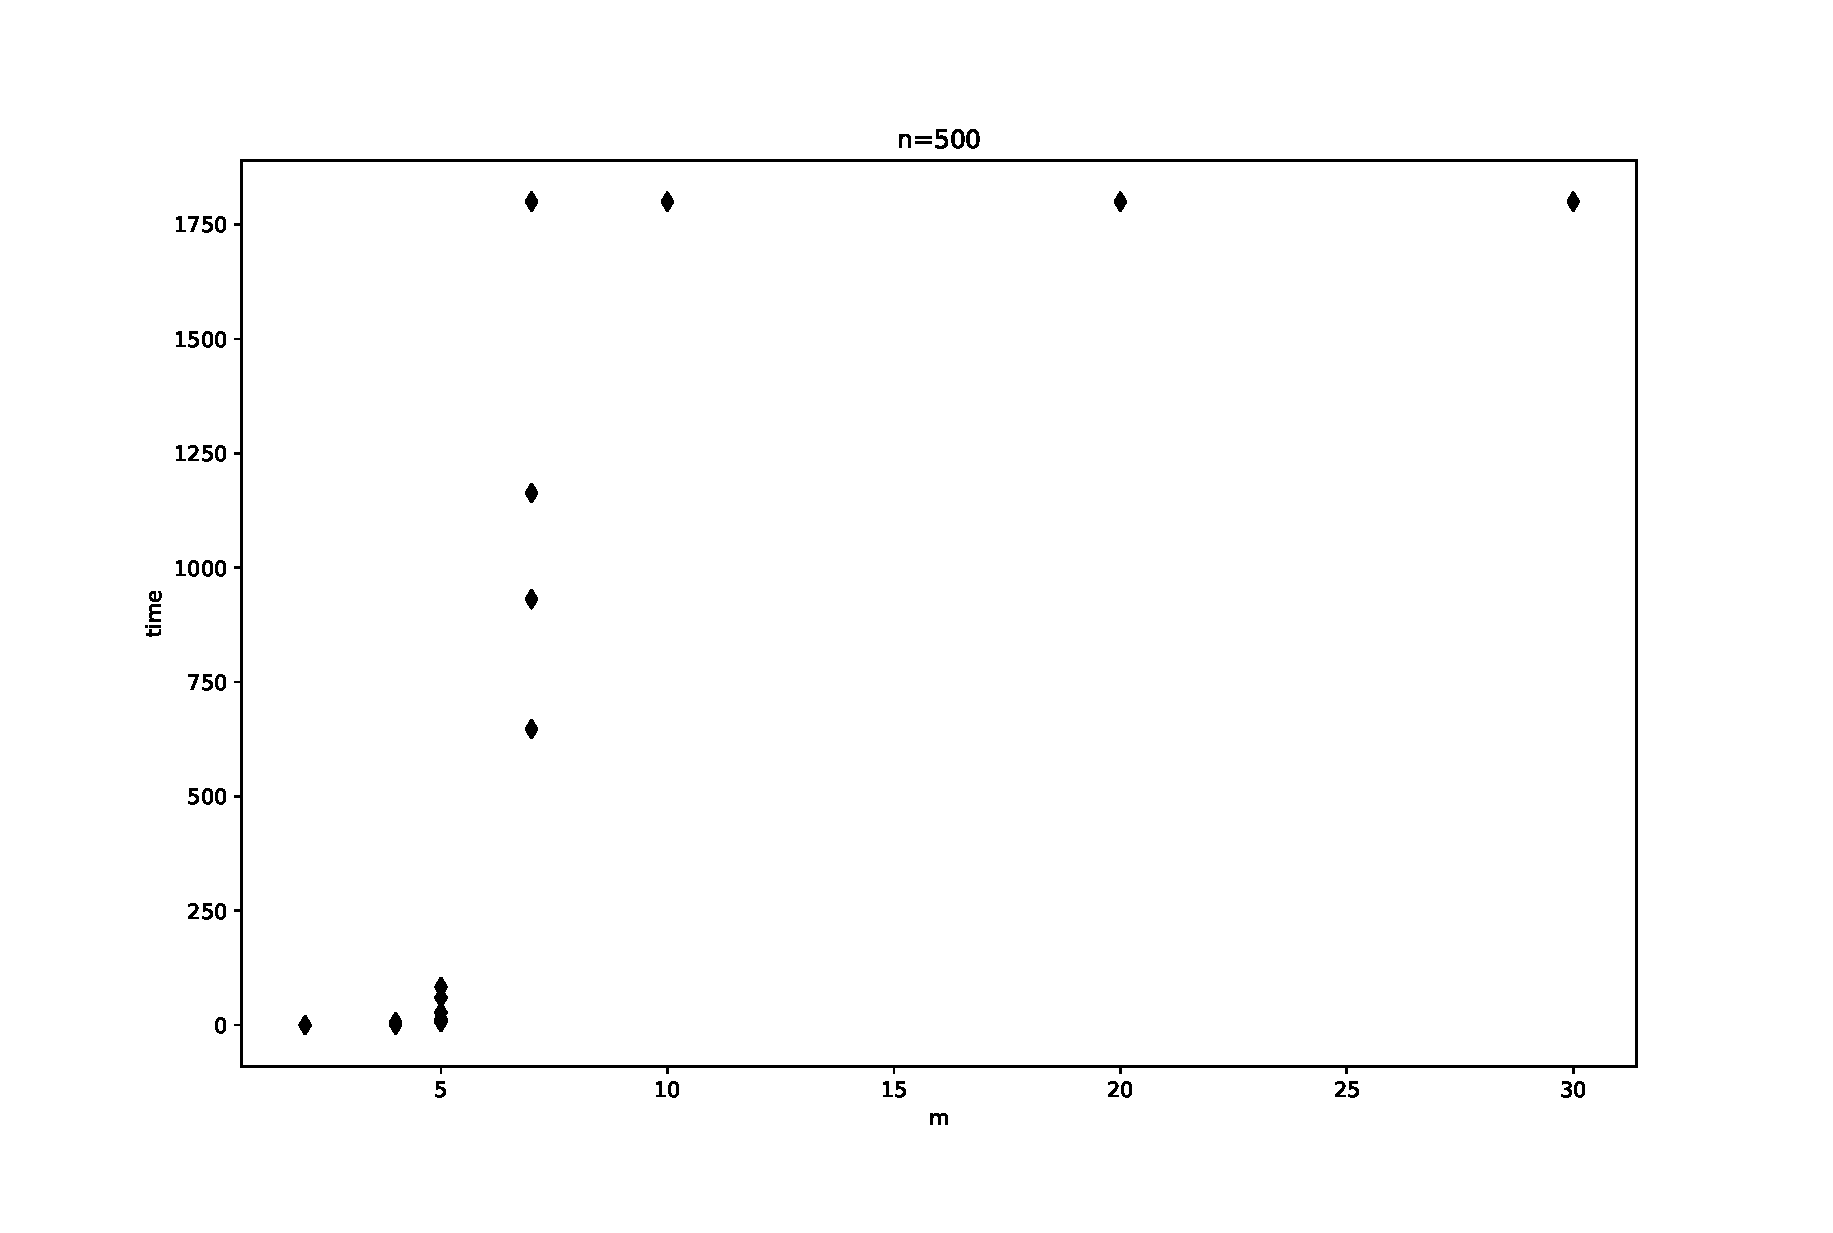
\includegraphics[width=\columnwidth]{images/bagm5.eps}
	     \end{subfigure}
		\end{subfigure}
        \caption{Andamento del tempo di risoluzione in funzione del parametro $m$, che rappresenta il numero di nodi esistenti a cui è collegato un nuovo nodo nel processo iterativo di costruzione del grafo, per valori di $n$ fissati.}
        \label{fig:bagma}
\end{figure}

Infine, anche per i risultati ottenuti dall'analisi di grafi di Barabási-Albert è stata elaborata un'immagine tridimensionale per visualizzare l'andamento della complessità del problema di vertex cover associato all'istanza di grafo al variare di entrambi i parametri di generazione $m$ e $n$.
  \vspace{-1cm}  
\begin{figure}[h!]
     \centering
       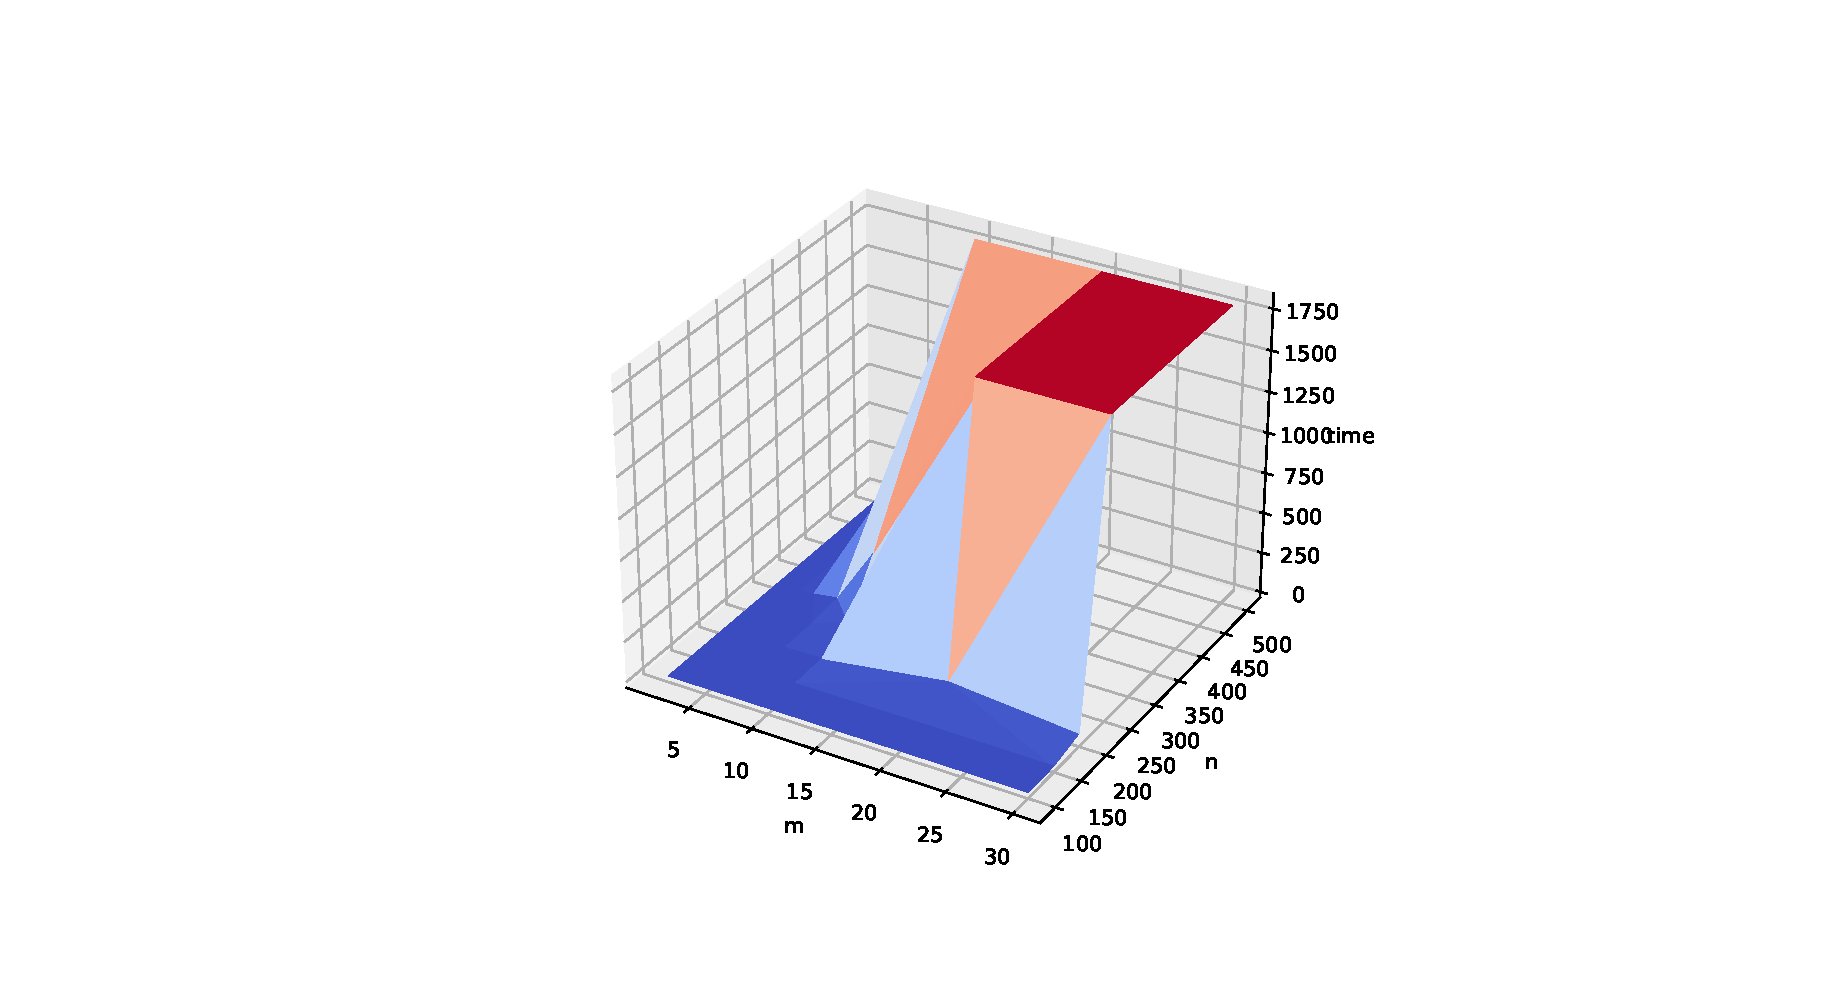
\includegraphics[scale=0.4]{images/bag-3d.eps}
       \vspace{-0.8cm}  
       \caption{Rappresentazione tridimensionale dell'andamento della complessità del problema di vertex cover per grafi di Barabási-Albert al variare dei parametri $m$ ed $n$. Anche in questo caso colori più caldi indicano una complessità maggiore, ed il colore rosso scuro è generalmente sinonimo di raggiungimento del time limit imposto al risolutore.}      
        \label{fig:bag3d}
\end{figure}